\documentclass[tikz, border = 1 cm]{standalone}

%%%%%%%%%%%%%%
\usepackage{tikz}
\usetikzlibrary{calc}
%%%%%%%%%%%%%%

%%%%%%%%%%%%%%
\definecolor{blue4}{RGB}{178,231,248}
\definecolor{gray4}{RGB}{201,203,206}
\definecolor{orange4}{RGB}{255,216,192}
%%%%%%%%%%%%%%

%%%%%%%%%%%%%%
%%%%%%%%%%%%%%
%%%%%%%%%%%%%%
\begin{document}

%%%%%%%%%%%%%%
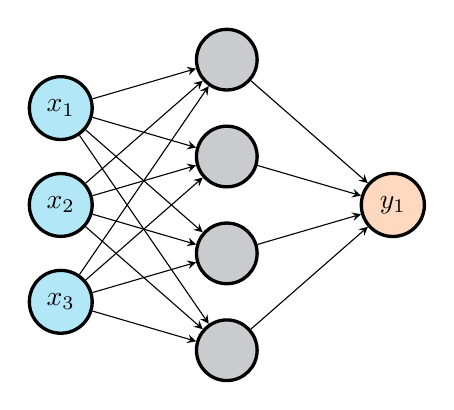
\begin{tikzpicture}[	netnode/.style=		{circle, inner sep=0pt, text width=22pt, align=center, very thick},
				inputnode/.style=	{netnode, fill=blue4, draw=black},
				hiddennode/.style=	{netnode, fill=gray4, draw=black},
				outputnode/.style=	{netnode, fill=orange4, draw=black},
				signal/.style=		{arrows={-stealth}, draw=black}]
	\def\nodedist{35pt}
	\def\layerdist{60pt}
    
	\foreach \y in {1,...,3}
		\node[inputnode] (I\y) at (0,-\y*\nodedist) {$x_\y$};  
	\foreach \y in {1,...,4}
		\node[hiddennode] (H1\y) at ($(\layerdist,-\y*\nodedist) +(0, 0.5*\nodedist)$) {};
	\foreach \y in {1,...,1}
		\node[outputnode] (O\y) at ($0.5*(H11) + 0.5*(H12) + (\layerdist, -\y*\nodedist)$) {$y_\y$};

	\foreach \dest in {1,...,4}
		\foreach \source in {1,...,3}
			\draw[signal] (I\source) -- (H1\dest);
	\foreach \dest in {1,...,1}
		\foreach \source in {1,...,4}
			\draw[signal] (H1\source) edge (O\dest);
\end{tikzpicture}
%%%%%%%%%%%%%%

\end{document}